\section{Question 2}

\subsection{The Question}

Write a Python program that:
\begin{itemize}
\item takes one argument, like "Old Dominion" or "Virginia Tech"
\item  takes another argument specified in seconds (e.g., "60" for 
     one minute).
 \item takes a URI as a third argument: 

     \url{http://sports.yahoo.com/college-football/scoreboard/}
    
    or

     \url{http://sports.yahoo.com/college-football/scoreboard/?week=2&conf=all}
    
 or

     \url{http://sports.yahoo.com/college-football/scoreboard/?week=1&conf=72}

     etc.
 \item dereferences the URI, finds the game corresponding to the team
     argument, prints out the current score (e.g., "Old Dominion 27, 
     East Carolina 17), sleeps for the specified seconds, and then
     repeats (until control-C is hit).
\end{itemize}


\subsection{The Answer}

The beautiful soup library converts the complex HTML file tree to a python object tree that contains methods that permit the easy traversal and search of the tree. Initially the structure site of interest was understood by inspecting the page in a web client, i.e. Chrome. This way the specific tags of interest can be easily known without exploring the entire tree in python. Then by targeting these tags we can find all of their instances and find the one that matched our search. Therefore all the away team tags are searched for the team of interest, then all the home teams. Once the tag of interest is found we can use it as a frame of reference to find the other items we need. 

Of course there is a condition for the possibility that the desired team was not available. Assuming it was located its sibling and parents can be used to easy find the location of the opponent team and score without searching the entire tree again. 
The time library allows for a sleep to be inserted at any point in the code.  

\lstset{
    language=bash,
    label=code:q1_bash,
    caption={Command line input}
}

\lstinputlisting{../q2/getScore.sh}


\lstset{
    language=python,
    label=code:correction_8.5,
    caption={Python code implementing the score search}
}

\lstinputlisting{../q2/urlCode.py}

\begin{figure}
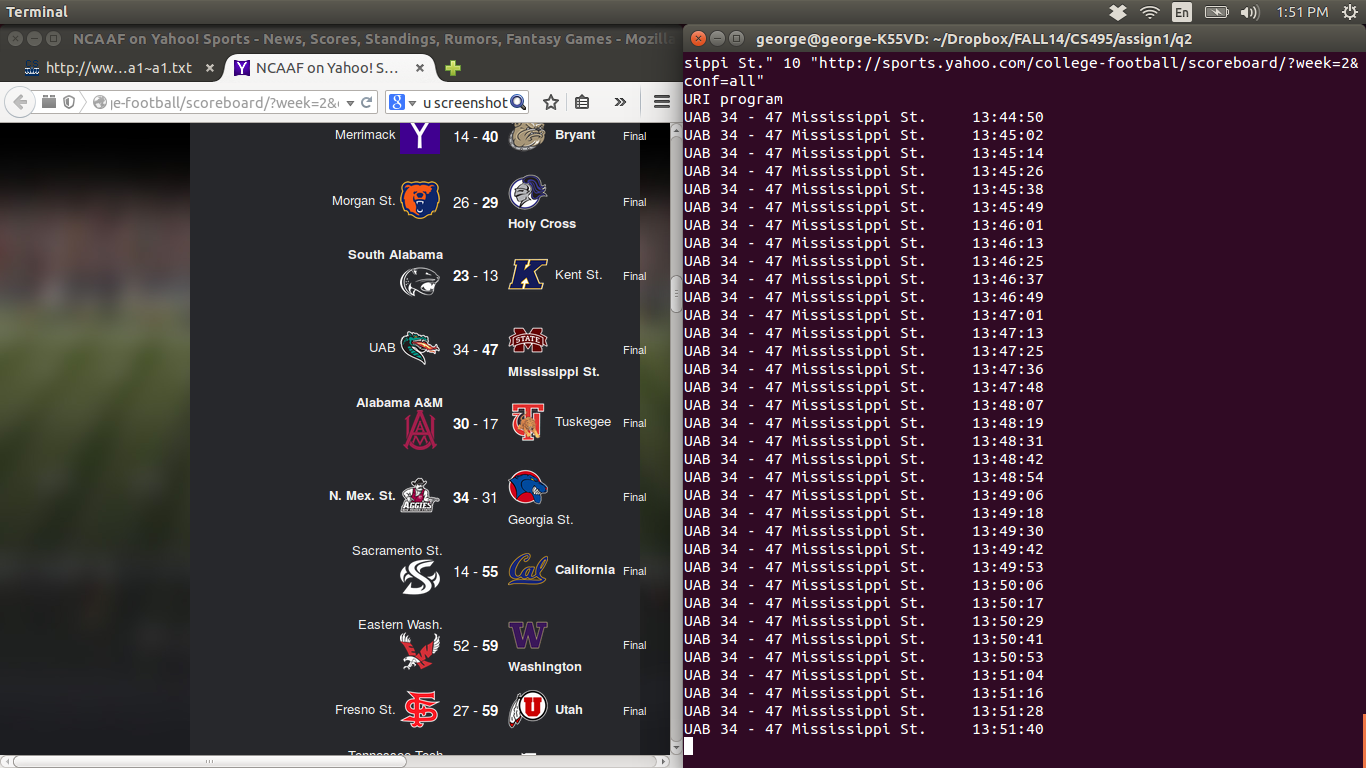
\includegraphics[width=\textwidth]{figures/scoreScreen}
 \caption{Screenshot of the script execution}
\end{figure}
